\PassOptionsToPackage{unicode=true}{hyperref} % options for packages loaded elsewhere
\PassOptionsToPackage{hyphens}{url}
%
\documentclass[]{book}
\usepackage{lmodern}
\usepackage{amssymb,amsmath}
\usepackage{ifxetex,ifluatex}
\usepackage{fixltx2e} % provides \textsubscript
\ifnum 0\ifxetex 1\fi\ifluatex 1\fi=0 % if pdftex
  \usepackage[T1]{fontenc}
  \usepackage[utf8]{inputenc}
  \usepackage{textcomp} % provides euro and other symbols
\else % if luatex or xelatex
  \usepackage{unicode-math}
  \defaultfontfeatures{Ligatures=TeX,Scale=MatchLowercase}
\fi
% use upquote if available, for straight quotes in verbatim environments
\IfFileExists{upquote.sty}{\usepackage{upquote}}{}
% use microtype if available
\IfFileExists{microtype.sty}{%
\usepackage[]{microtype}
\UseMicrotypeSet[protrusion]{basicmath} % disable protrusion for tt fonts
}{}
\IfFileExists{parskip.sty}{%
\usepackage{parskip}
}{% else
\setlength{\parindent}{0pt}
\setlength{\parskip}{6pt plus 2pt minus 1pt}
}
\usepackage{hyperref}
\hypersetup{
            pdftitle={Recettes des 4 saisons},
            pdfauthor={Honorine et Jonas},
            pdfborder={0 0 0},
            breaklinks=true}
\urlstyle{same}  % don't use monospace font for urls
\usepackage{longtable,booktabs}
% Fix footnotes in tables (requires footnote package)
\IfFileExists{footnote.sty}{\usepackage{footnote}\makesavenoteenv{longtable}}{}
\usepackage{graphicx,grffile}
\makeatletter
\def\maxwidth{\ifdim\Gin@nat@width>\linewidth\linewidth\else\Gin@nat@width\fi}
\def\maxheight{\ifdim\Gin@nat@height>\textheight\textheight\else\Gin@nat@height\fi}
\makeatother
% Scale images if necessary, so that they will not overflow the page
% margins by default, and it is still possible to overwrite the defaults
% using explicit options in \includegraphics[width, height, ...]{}
\setkeys{Gin}{width=\maxwidth,height=\maxheight,keepaspectratio}
\setlength{\emergencystretch}{3em}  % prevent overfull lines
\providecommand{\tightlist}{%
  \setlength{\itemsep}{0pt}\setlength{\parskip}{0pt}}
\setcounter{secnumdepth}{5}
% Redefines (sub)paragraphs to behave more like sections
\ifx\paragraph\undefined\else
\let\oldparagraph\paragraph
\renewcommand{\paragraph}[1]{\oldparagraph{#1}\mbox{}}
\fi
\ifx\subparagraph\undefined\else
\let\oldsubparagraph\subparagraph
\renewcommand{\subparagraph}[1]{\oldsubparagraph{#1}\mbox{}}
\fi

% set default figure placement to htbp
\makeatletter
\def\fps@figure{htbp}
\makeatother

\usepackage{booktabs}
\usepackage{amsthm}
\makeatletter
\def\thm@space@setup{%
  \thm@preskip=8pt plus 2pt minus 4pt
  \thm@postskip=\thm@preskip
}
\makeatother

\usepackage{color}
\usepackage{framed}
\setlength{\fboxsep}{.8em}

%\newenvironment{FOO}{
%  \definecolor{shadecolor}{rgb}{0, 0, 0}  % black
%  \color{white}
%  \begin{shaded}}
% {\end{shaded}}

\usepackage{tcolorbox}

\newtcolorbox{sucrebox}{
  colback=gray,
  colframe=orange,
  coltext=black,
  boxsep=5pt,
  arc=4pt}
  
\newtcolorbox{salebox}{
  colback=gray,
  colframe=orange,
  coltext=black,
  boxsep=5pt,
  arc=4pt}
\usepackage[]{natbib}
\bibliographystyle{plainnat}

\title{Recettes des 4 saisons}
\author{Honorine et Jonas}
\date{2020-05-02}

\begin{document}
\maketitle

{
\setcounter{tocdepth}{1}
\tableofcontents
}
\hypertarget{Pruxe9ambule}{%
\chapter*{Préambule}\label{Pruxe9ambule}}
\addcontentsline{toc}{chapter}{Préambule}

Ceci est notre livre de recettes

\begin{quote}
La perfection est atteinte, non pas lorsqu'il n'y a plus rien à ajouter, mais lorsqu'il n'y a plus rien à retirer

Antoine de Saint-Exupéry
\end{quote}

\hypertarget{hiver}{%
\chapter*{Hiver}\label{hiver}}
\addcontentsline{toc}{chapter}{Hiver}

\hypertarget{saluxe9}{%
\section*{Salé}\label{saluxe9}}
\addcontentsline{toc}{section}{Salé}

\hypertarget{linguines-citron-et-coriandre}{%
\subsection*{\texorpdfstring{{Linguines citron et coriandre}}{Linguines citron et coriandre}}\label{linguines-citron-et-coriandre}}
\addcontentsline{toc}{subsection}{{Linguines citron et coriandre}}

\begin{salebox}
\textbf{2 personnes \textbar{} Temps préparation : 10 min \textbar{}
Temps cuisson : 10 min}

Plat de pâtes simple et rapide mais percutant !
\end{salebox}

\textbf{Ingrédients}

\begin{itemize}
\tightlist
\item
  250 g de linguines (au pire des spaghetti)
\item
  1 à 2 citrons bios
\item
  2 gousses d'ail
\item
  Quelques brins de coriandre
\item
  Beurre
\item
  Crème
\end{itemize}

\textbf{Consignes}

\begin{itemize}
\tightlist
\item
  Eplucher l'ail et la couper en petits morceaux
\item
  Faire fondre un peu de beurre dans une casserole et y faire revenir à feu doux le zeste du/des citrons et l'ail
\item
  Faire chauffer l'eau des pâtes (dans une autre casserole bien sûr)
\item
  Rajouter le jus de citron et 5 à 6 cs de crème dans la sauce. Laisser s'amalgamer à feu doux
\item
  Cuire les pâtes, 1 à 2 min de moins que nécessaire
\item
  Mettre 1 ou 2 cs d'eau de cuisson des pâtes dans la sauce
\item
  Égoutter les pâtes et les mettre directement dans la sauce où elles finiront de cuire en s'imbibant de sauce.
\item
  Ciseler la coriandre et l'ajouter
\item
  Assaisonner selon les gouts et servir
\end{itemize}

\begin{center}\rule{0.5\linewidth}{0.5pt}\end{center}

\hypertarget{couscous-boulette-vuxe9guxe9tarien}{%
\subsection*{\texorpdfstring{{Couscous boulette végétarien}}{Couscous boulette végétarien}}\label{couscous-boulette-vuxe9guxe9tarien}}
\addcontentsline{toc}{subsection}{{Couscous boulette végétarien}}

\begin{salebox}
\textbf{\textasciitilde{}15 boulettes \textbar{} Temps préparation : 30
min \textbar{} Temps cuisson : 20 min}

Pour un plat chaleureux et convivial au coeur de l'hiver.
\end{salebox}

\textbf{Ingrédients}

\begin{itemize}
\tightlist
\item
  250 g de champignons de Paris
\item
  2 gousses d'ail
\item
  1 oignon
\item
  100 g d'amandes
\item
  120 g de pain rassis
\item
  10 branches de persil
\item
  2 œufs
\end{itemize}

\textbf{Consignes}

\begin{itemize}
\tightlist
\item
  Hacher très finement les champignons, l'oignon et l'ail
\item
  Les faire revenir dans un peu d'huile d'olive pendant 5 min
\item
  Mixer les amandes et le pain rassis
\item
  Ciseler le persil
\item
  Dans un saladier, mettre tous les ingrédients et ajouter les œufs
\item
  Mélanger, assaisonner et mettre au réfrigérateur (facultatif)
\item
  Préchauffer le four à 180°C et préparer une feuille de papier sulfurisé sur la plaque
\item
  Former une quinzaine de boulettes, poser les sur la plaque et les badigeonner d'un peu d'huile avec un pinceau
\item
  Enfourner pour une vingtaine de minutes
\item
  Servir avec des légumes (courges, patates douces, navets, carottes, pois chiches, blettes selon les envies et la saison) cuits dans du concentré de tomates et des épices, et de la semoule
\end{itemize}

\begin{center}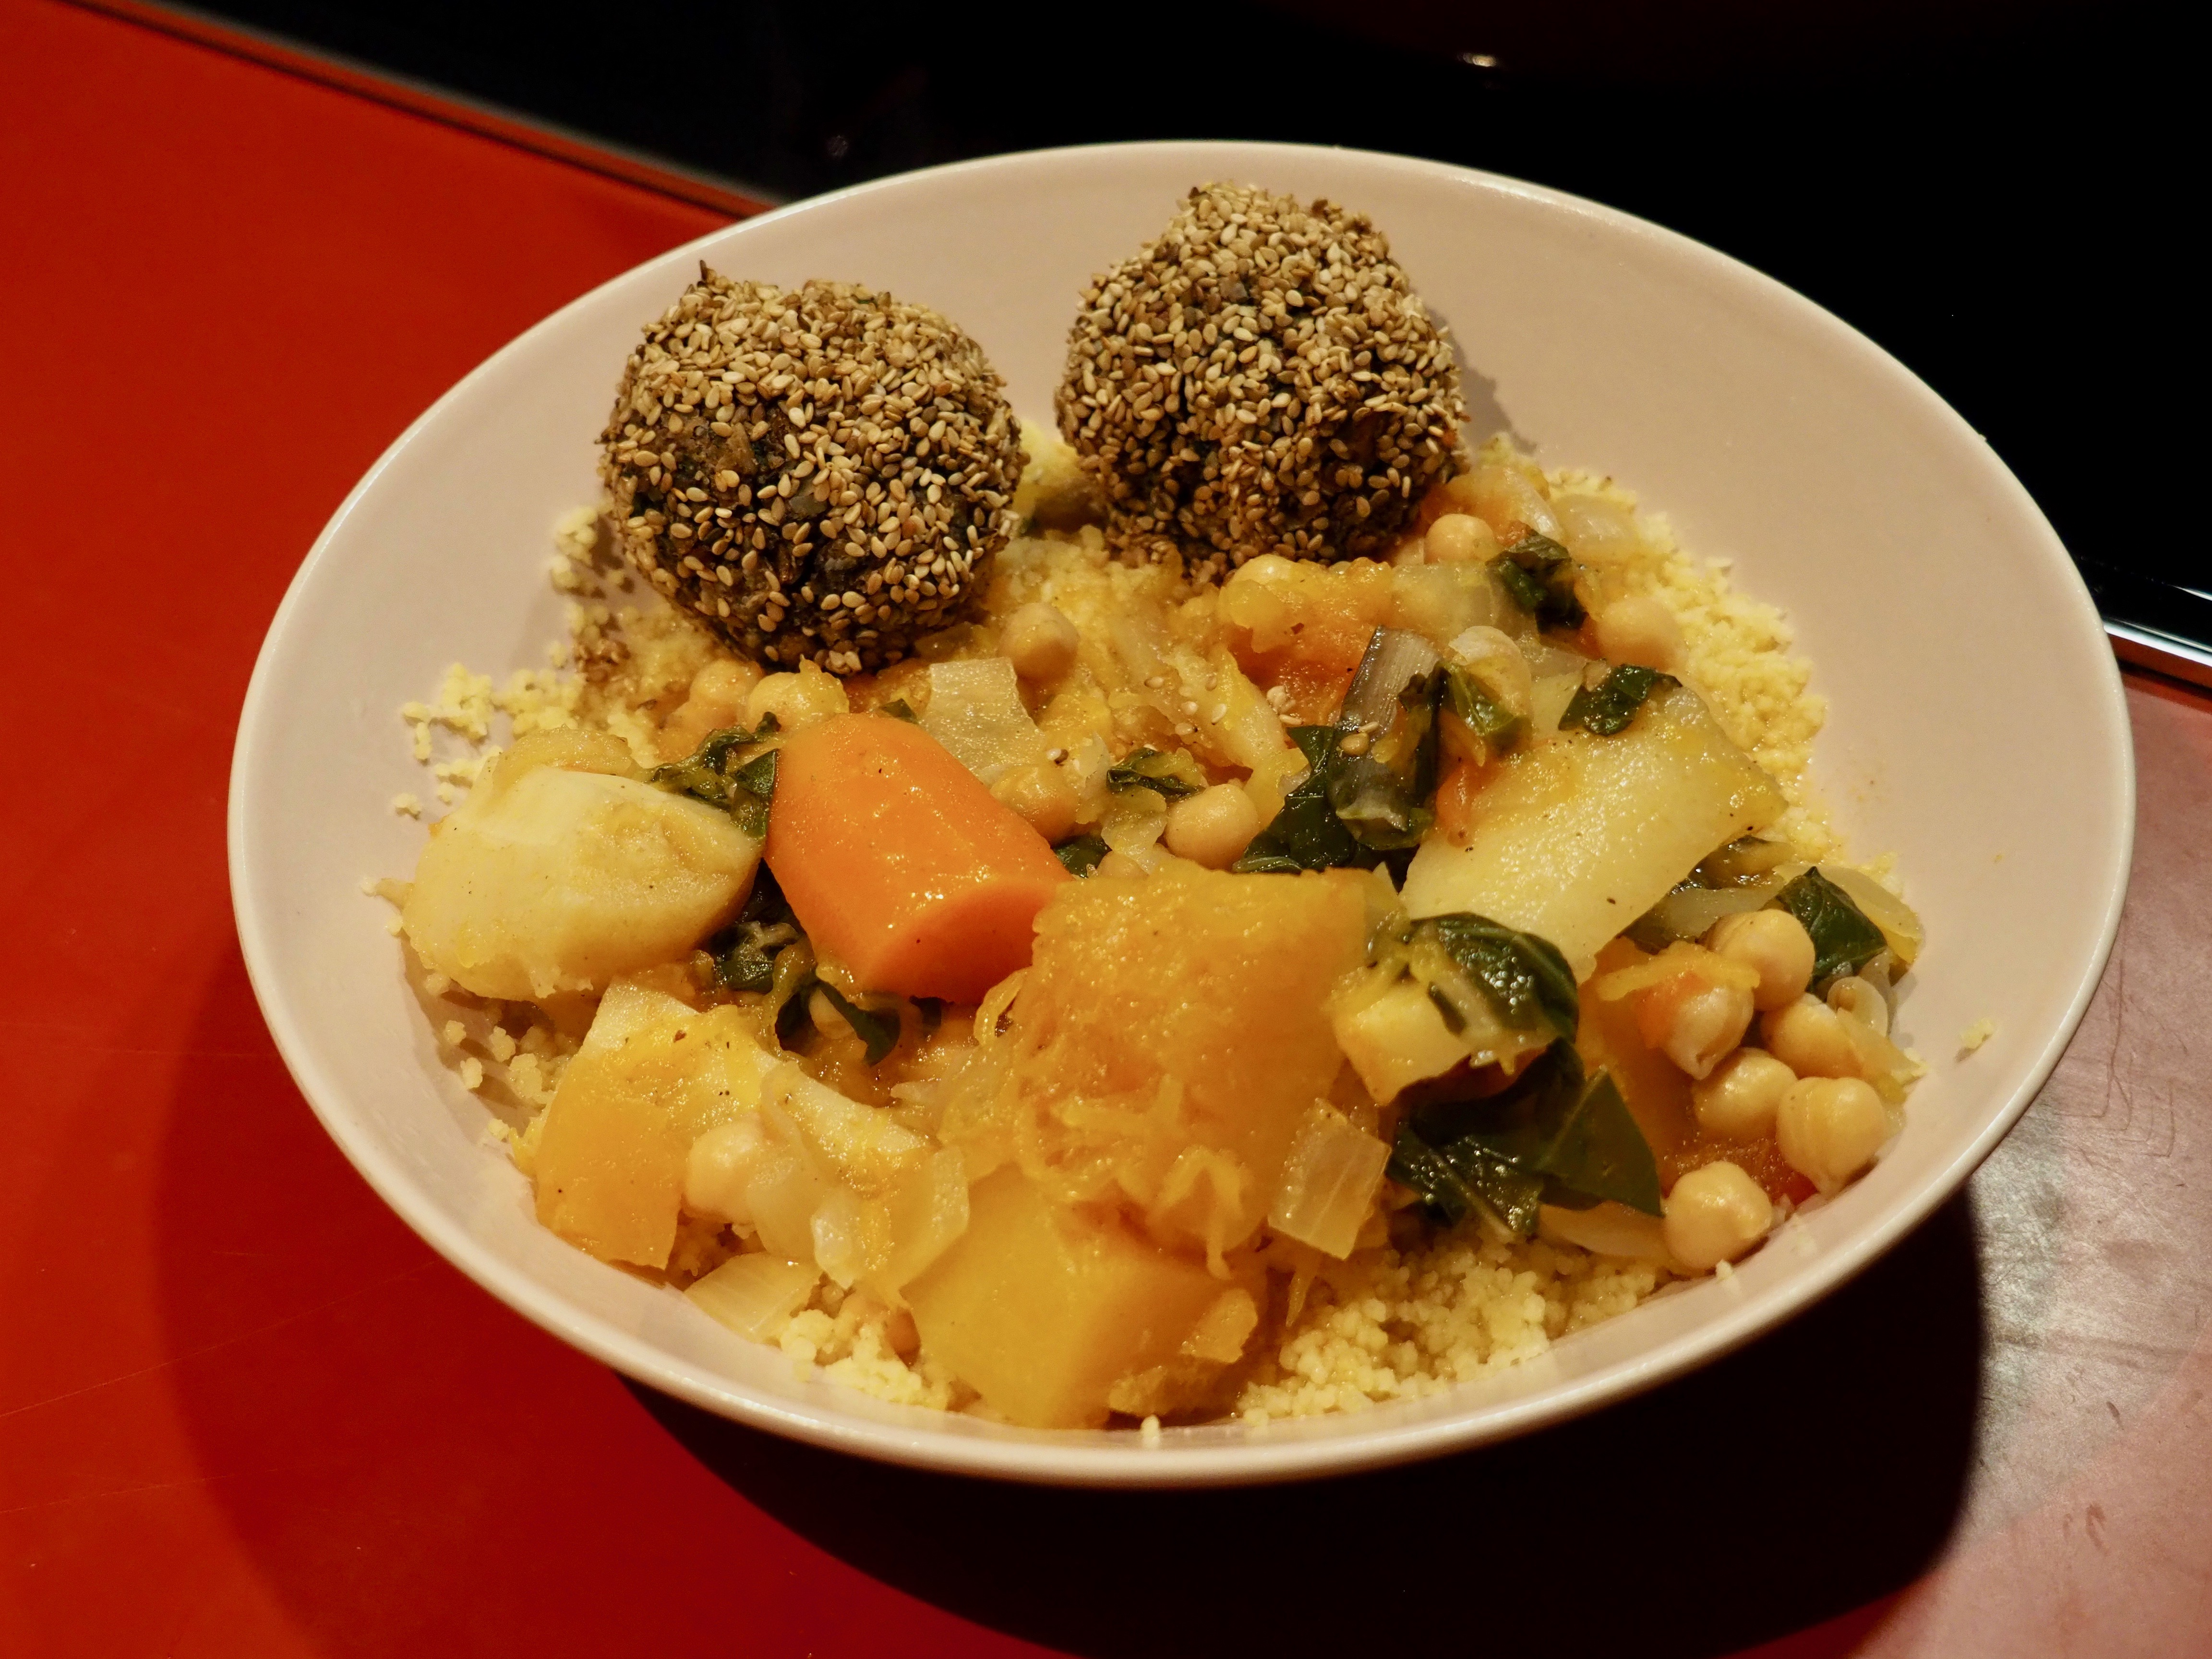
\includegraphics[width=0.9\linewidth]{photos/couscous} \end{center}

\begin{center}\rule{0.5\linewidth}{0.5pt}\end{center}

\hypertarget{risotto-pomme-noix-gorgonzola}{%
\subsection*{\texorpdfstring{{Risotto pomme noix gorgonzola}}{Risotto pomme noix gorgonzola}}\label{risotto-pomme-noix-gorgonzola}}
\addcontentsline{toc}{subsection}{{Risotto pomme noix gorgonzola}}

\begin{salebox}
\textbf{3 personnes \textbar{} Temps préparation : 10 min \textbar{}
Temps cuisson : 30 min}

Un risotto gourmand et fruité
\end{salebox}

\textbf{Ingrédients}

\begin{itemize}
\tightlist
\item
  250 g riz à risotto
\item
  1 oignon
\item
  2 pommes
\item
  80 g de gorgonzola
\item
  20 g de noix
\item
  1 peu de vin blanc pour déglacer
\end{itemize}

\textbf{Consignes}

\begin{itemize}
\tightlist
\item
  Peler et couper l'oignon
\item
  Faire chauffer de l'eau pour le bouillon
\item
  Les faire revenir dans un peu d'huile d'olive pendant 5 min puis ajouter le riz
\item
  Une fois le riz transparent, déglacer au vin blanc
\item
  Une fois le vin blanc évaporé, commencer à rajouter de l'eau petit à petit jusqu'à ce que le riz soit cuit
\item
  Peler la pomme (pour faire un peu de déco comme sur la photo garder une longue épluchure)
\item
  Un peu avant qu'il soit cuit, ajouter les pommes préalablement coupées en dés
\item
  Une fois le riz cuit, ajouter les noix et le gorgonzola
\item
  Laisser cuire 5 min puis servir
\end{itemize}

\begin{center}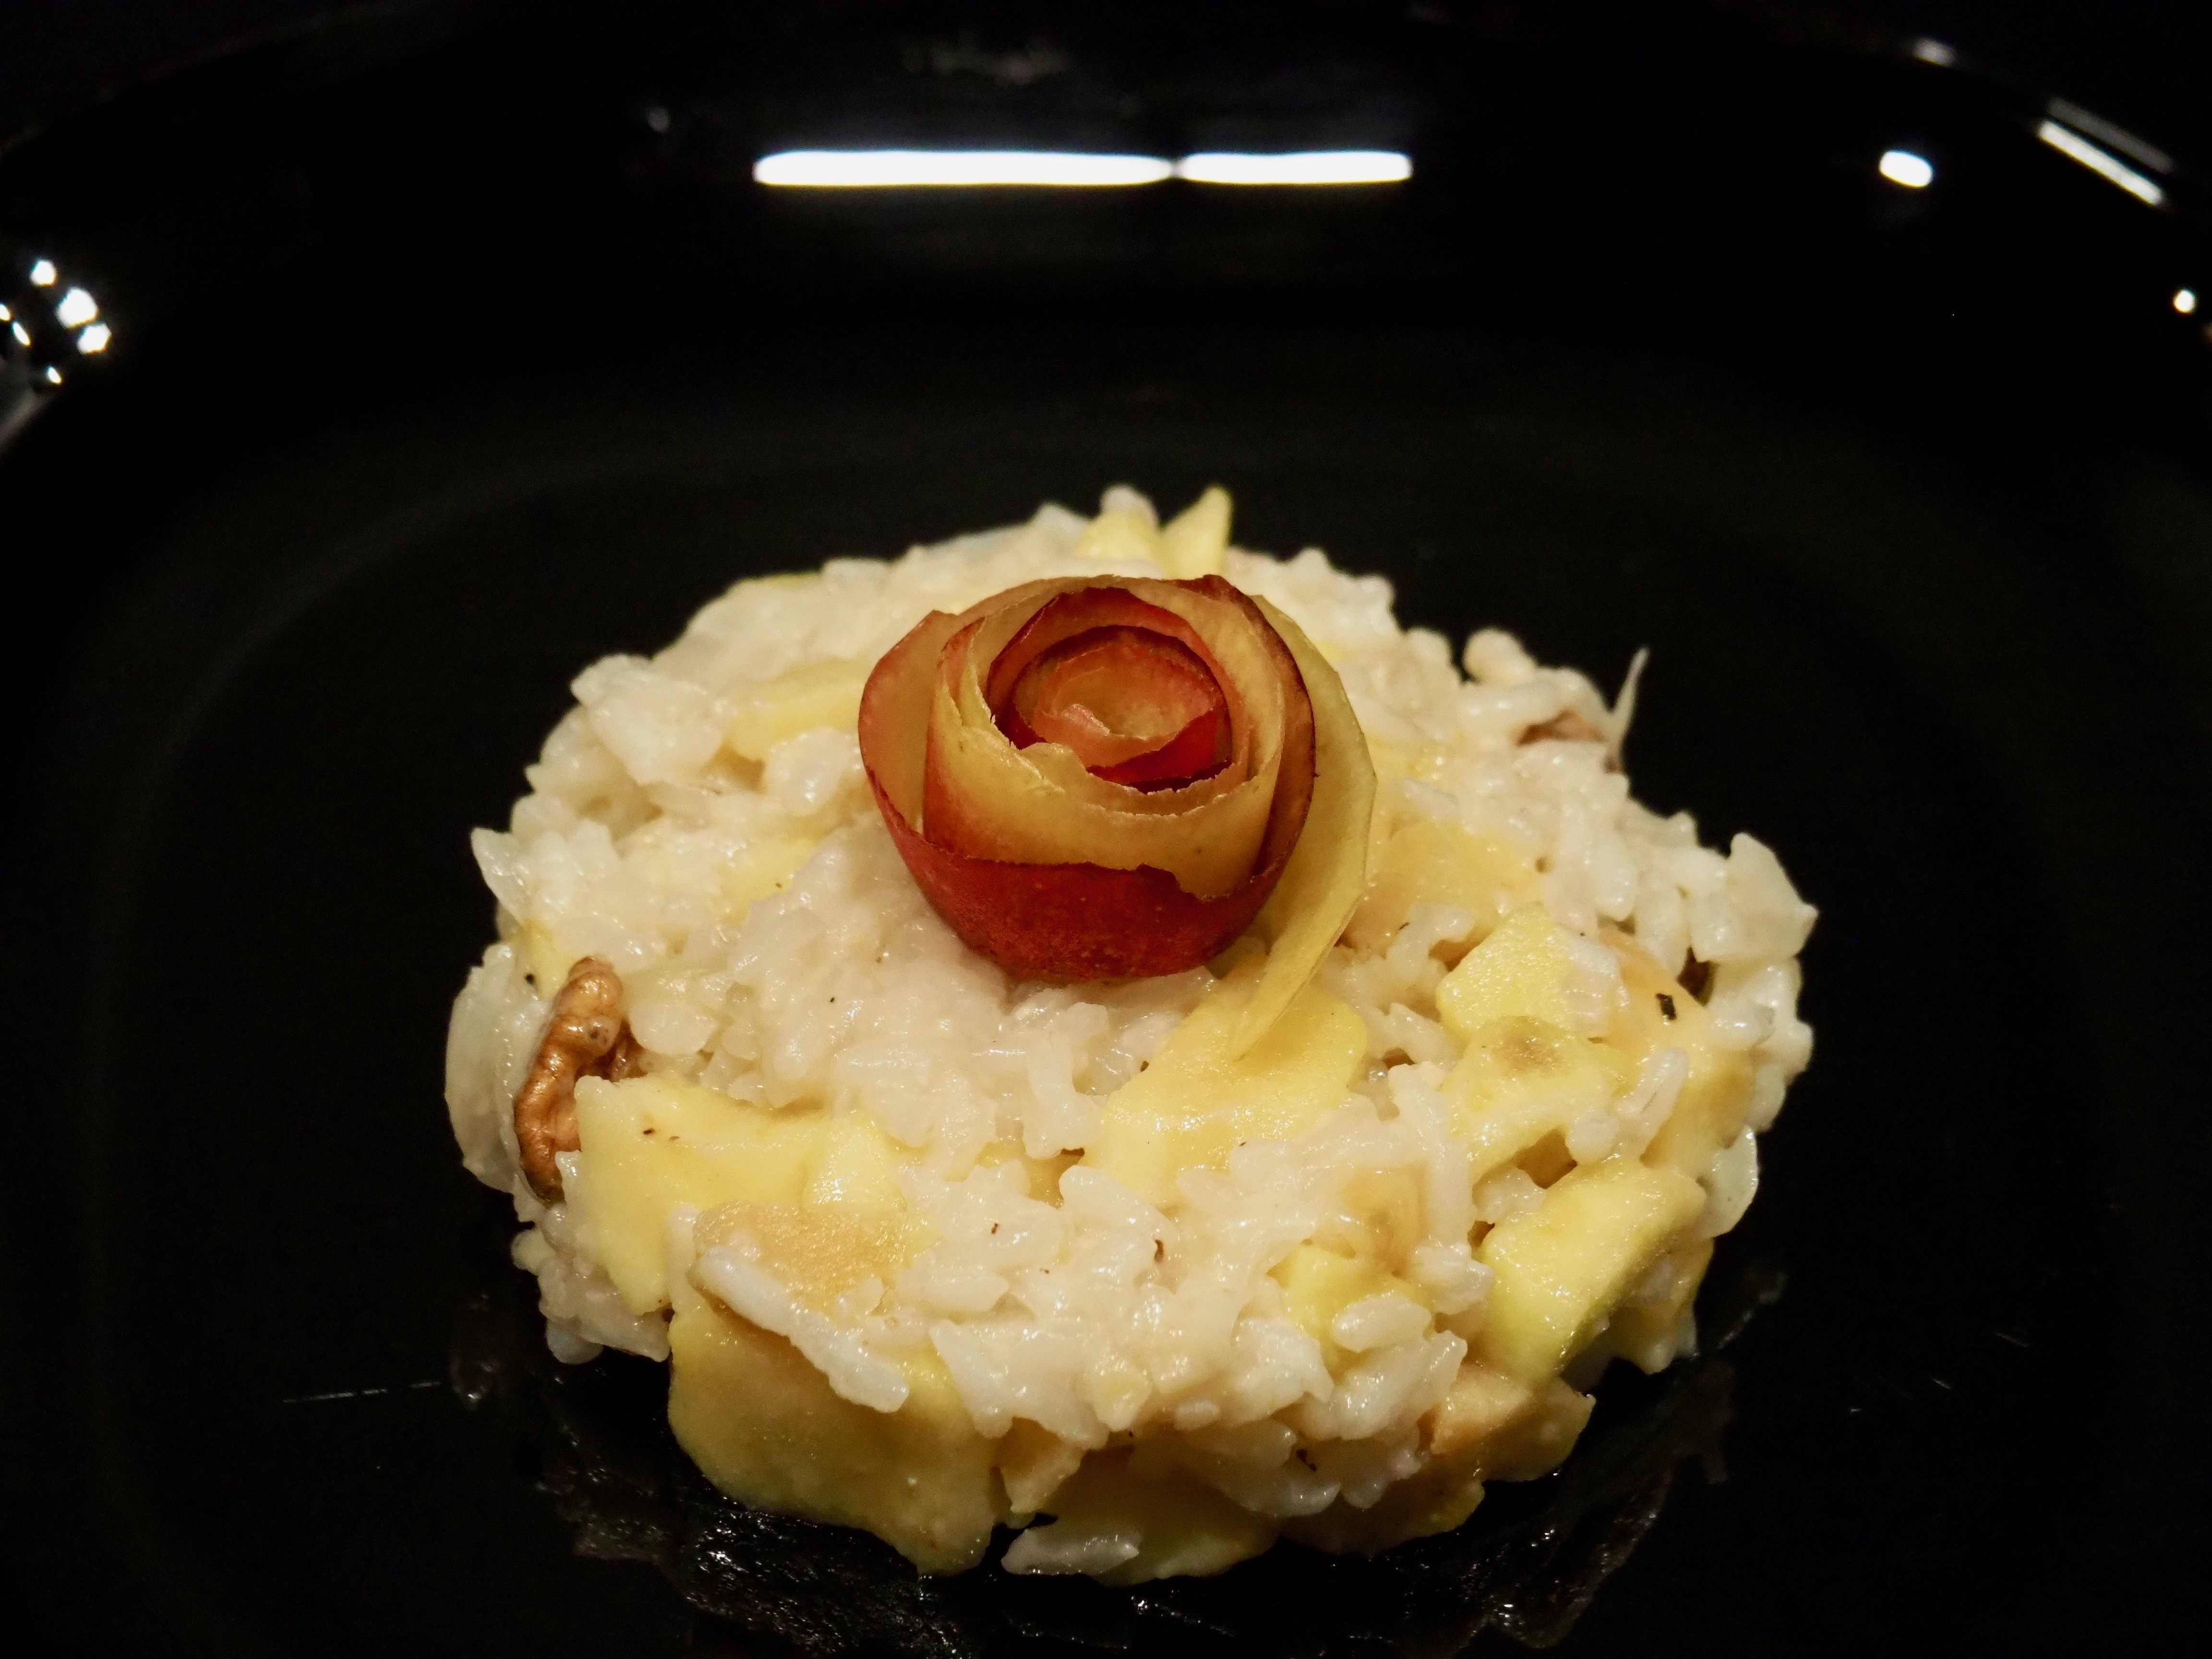
\includegraphics[width=0.9\linewidth]{photos/risotto-gorgonzola} \end{center}

\begin{center}\rule{0.5\linewidth}{0.5pt}\end{center}

\hypertarget{steak-vuxe9guxe9tarien}{%
\subsection*{\texorpdfstring{{Steak végétarien}}{Steak végétarien}}\label{steak-vuxe9guxe9tarien}}
\addcontentsline{toc}{subsection}{{Steak végétarien}}

\begin{salebox}
\textbf{\textasciitilde{}10 steaks \textbar{} Temps préparation : 25 min
\textbar{} Temps cuisson : 25 min}

Des steaks végétariens pour garnir différentes recettes de burgers
(pomme/chèvre ; comté/champignons)
\end{salebox}

\textbf{Ingrédients}

\begin{itemize}
\tightlist
\item
  250 g de pois chiches en boite
\item
  250 g de haricot rouges en boite
\item
  1 petite boite de maïs
\item
  1 oignon
\item
  1 poivron
\item
  1 carotte
\item
  3 gousses d'ail
\item
  90 g de flocons d'avoine
\item
  50 g de chapelure ou de pain rassis
\item
  2 œufs
\item
  2 cs de sauce soja
\item
  Épices : cumin, curry, piment\ldots{} Au choix !
\end{itemize}

\textbf{Consignes}

\begin{itemize}
\tightlist
\item
  Mixer grossièrement les pois chiches et les haricots rouges (sans les réduire en purée)
\item
  Faire de même avec la carotte, le poivron, l'oignon et l'ail (ou les couper très finement)
\item
  Faire revenir l'oignon et l'ail dans un peu d'huile d'olive
\item
  Rajouter le poivron et la carotte et attendre qu'ils soient cuits
\item
  Dans un saladier, mélanger les légumes, les légumineuses, le maïs, les flocons d'avoines, les œufs
\item
  Assaisonner selon les envies et mélanger à la main
\item
  Préchauffer le four à 180°C
\item
  Former des galettes d'environ 1 cm d'épaisseur et les déposer sur un papier sulfurisé sur une plaque allant au four
\item
  Enfourner une quinzaine de minutes puis les retourner
\item
  Laisser encore cuire entre 5 et 10 min et sortir du four
\item
  Déguster immédiatement ou les congeler
\end{itemize}

\begin{center}\rule{0.5\linewidth}{0.5pt}\end{center}

\hypertarget{riz-sautuxe9-aux-crevettes-et-ananas}{%
\subsection*{\texorpdfstring{{Riz sauté aux crevettes et ananas}}{Riz sauté aux crevettes et ananas}}\label{riz-sautuxe9-aux-crevettes-et-ananas}}
\addcontentsline{toc}{subsection}{{Riz sauté aux crevettes et ananas}}

\begin{salebox}
\textbf{3 personnes \textbar{} Temps préparation : 30 min \textbar{}
Temps cuisson : 30 min}

Un voyage en Asie pour pas cher !
\end{salebox}

\textbf{Ingrédients}

\begin{itemize}
\tightlist
\item
  250g de riz basmati ou thaï
\item
  1 ananas (2 si présentation dans un demi ananas)
\item
  1 oignon
\item
  500 g de crevettes non décortiquées
\item
  Quelques brins de coriandre
\item
  Sauce soja
\end{itemize}

\textbf{Consignes}

\begin{itemize}
\tightlist
\item
  Faire cuire le riz dans un grand volume d'eau selon les indications. Egoutter puis réserver
\item
  Décortiquer les crevettes (garder les têtes pour faire un bouillon ou une sauce) et les couper en tronçon de 3 cm environ. Réserver
\item
  Eplucher l'oignon et le couper
\item
  Pour l'ananas deux possibilités :

  \begin{itemize}
  \tightlist
  \item
    Pour pouvoir l'utiliser en déco (cf.~photo), le couper en deux dans le sens de la longueur. Prélever la chair de chaque moitié en veillant à ne pas abimer la coque
  \item
    L'éplucher classiquement en enlevant les yeux (mais les coques ne pourront pas servir)
  \end{itemize}
\item
  Oter le milieu dur de l'ananas et couper en cube de 3 cm de côté environ
\item
  Dans une sauteuse, mettre de l'huile à chauffer puis ajouter l'oignon et l'ananas. Faire cuire une dizaine de minutes à feu moyen. Réserver dans une assiette
\item
  Remettre un peu d'huile et faire chauffer. Saisir les crevettes à feu moyen puis déglacer à la sauce soja. Rajouter l'ananas et l'oignon et enfin le riz
\item
  Laissez cuire une dizaine de minutes et essayant de faire doré un peu le riz. Rajoutez un peu de sauce soja selon les gouts et ajuster l'assaisonnement. Un peu avant la fin de la cuisson, rajouter la coriandre préalablement lavée et triée
\item
  Servir dans les demis ananas ou bien simplement dans une assiette
\end{itemize}

\begin{center}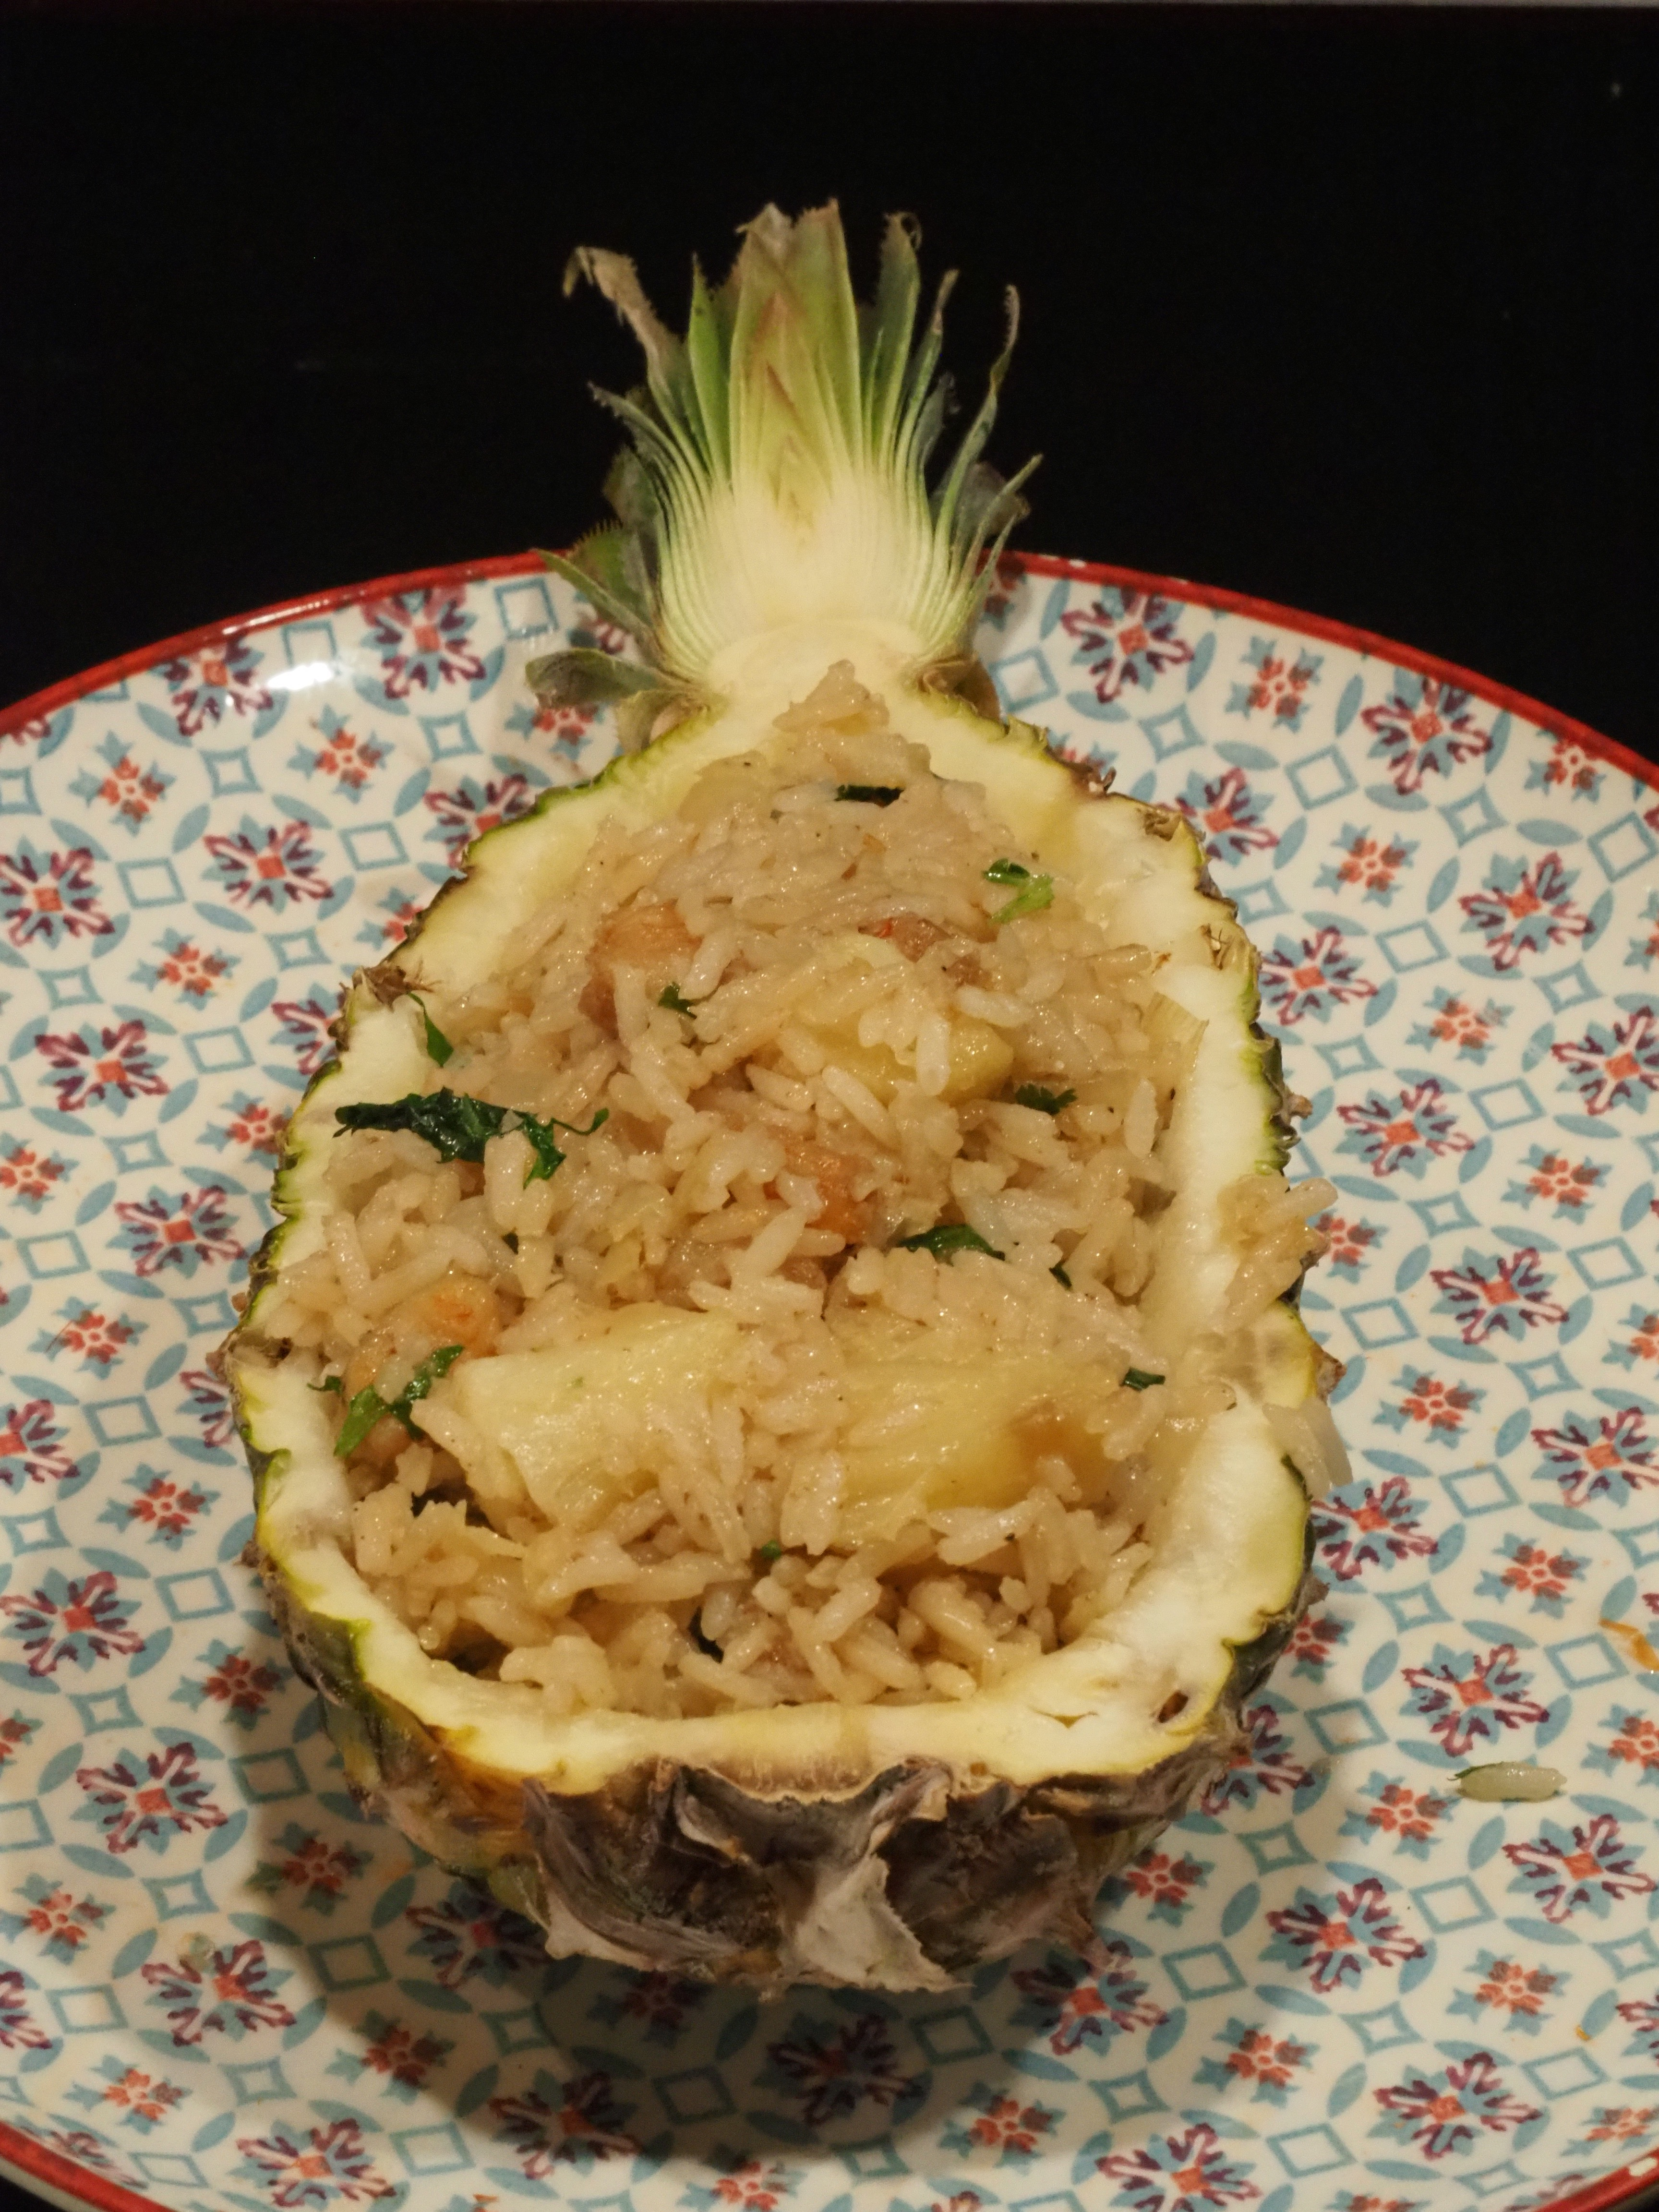
\includegraphics[width=0.9\linewidth]{photos/riz_saute} \end{center}

\begin{center}\rule{0.5\linewidth}{0.5pt}\end{center}

\hypertarget{sucruxe9}{%
\section*{Sucré}\label{sucruxe9}}
\addcontentsline{toc}{section}{Sucré}

\hypertarget{tartelettes-douces-amuxe8res-aux-framboises-et-pamplemousse}{%
\subsection*{\texorpdfstring{{Tartelettes douces-amères aux framboises et pamplemousse}}{Tartelettes douces-amères aux framboises et pamplemousse}}\label{tartelettes-douces-amuxe8res-aux-framboises-et-pamplemousse}}
\addcontentsline{toc}{subsection}{{Tartelettes douces-amères aux framboises et pamplemousse}}

\begin{sucrebox}
\textbf{4 tartelettes \textbar{} Temps préparation : 60 min \textbar{}
Temps cuisson : 40 min \textbar{} Temps repos : \textasciitilde{} 2h}

Tartelettes avec une bonne amertume, légèrement contrebalancées par la
douceur de la framboise
\end{sucrebox}

\textbf{Ingrédients}

\begin{itemize}
\tightlist
\item
  Pâte sablée ou sucrée pour 4 tartelettes
\item
  2 pamplemousses
\item
  60 g de sucre
\item
  2 g d'agar agar
\item
  150 g purée de framboise
\item
  45 g de jaune
\item
  60 g d'œuf
\item
  2 g de gélatine
\item
  60 g de beurre
\end{itemize}

\textbf{Consignes}

\begin{itemize}
\tightlist
\item
  Faire cuire les pâtes à blanc
\item
  Peler les pamplemousses et les couper grossièrement dans une casserole. Ajouter 40 g de sucre et faire chauffer jusqu'à obtenir une compotée suffisamment réduite
\item
  A la fin de la cuisson, rajouter 2 g d'agar agar puis refaire bouillir brièvement
\item
  Attendre que la compotée refroidisse et étaler dans les fonds de tarte
\item
  Pour le crémeux framboise, battre l'œuf, les jaunes et les 20 g de sucre restants jusqu'à ce que la préparation devienne mousseuse
\item
  Mettre la gélatine à réhydrater
\item
  Dans une casserole, faire chauffer la purée de framboise jusqu'à ébullition
\item
  Verser la moitié de la purée sur le mélange, mélanger et reverser dans la casserole
\item
  Chauffer en remuant jusqu'à ébullition, retirer du feu
\item
  Ajouter la gélatine et le beurre, mélanger jusqu'à incorporation
\item
  Verser sur la compotée de pamplemousse
\item
  Mettre au réfrigérateur jusqu'à ce que le crémeux soit pris
\item
  Possibilité de rajouter une meringue italienne avec les blancs restants
\end{itemize}

\begin{center}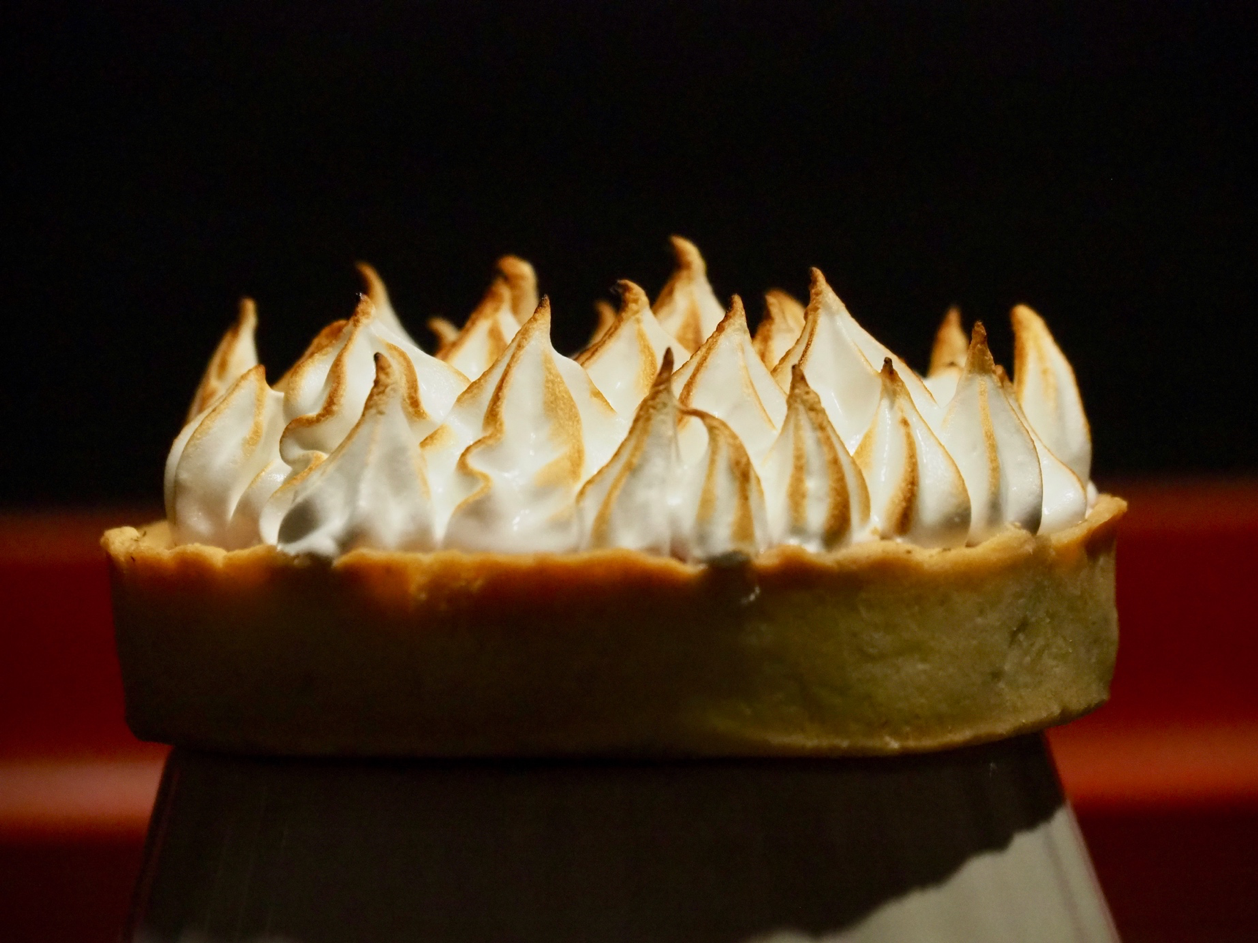
\includegraphics[width=0.9\linewidth]{photos/pamp1} \end{center}

\begin{center}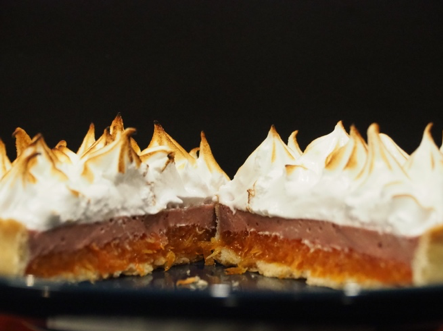
\includegraphics[width=0.9\linewidth]{photos/pamp2} \end{center}

\begin{center}\rule{0.5\linewidth}{0.5pt}\end{center}

\hypertarget{banana-bread}{%
\subsection*{\texorpdfstring{{Banana bread}}{Banana bread}}\label{banana-bread}}
\addcontentsline{toc}{subsection}{{Banana bread}}

\begin{sucrebox}
\textbf{8 personnes \textbar{} Temps préparation : 20 min \textbar{}
Temps cuisson : 50 min}

Toujours pratique pour un petit déjeuner
\end{sucrebox}

\textbf{Ingrédients}

\begin{itemize}
\tightlist
\item
  4/5 bananes bien mûres
\item
  40 g d'huile de coco
\item
  20 g de beurre
\item
  70 g de sucre
\item
  175 g de farine (100 \% blé ou mélange de farines)
\item
  3 œufs
\item
  ½ sachet de levure chimique
\item
  Garniture au choix : pépites de chocolat, fruits secs, graines, noisettes, amandes\ldots{}
\end{itemize}

\textbf{Consignes}

\begin{itemize}
\tightlist
\item
  Mélanger le beurre, l'huile de coco et le sucre et travailler jusqu'à obtenir une texture crémeuse.
\item
  Séparer les blancs des jaunes, incorporer les jaunes au mélange précédant
\item
  Écraser les bananes à la fourchette (ou mixer), et les incorporer
\item
  Ajouter la farine et la levure. Mélanger
\item
  Faire monter les blancs en neige ferme et les incorporer sans les casser avec une cuillère en bois
\item
  Ajouter la garniture choisie
\item
  Verser le tout dans un moule à cake préalablement beurré. Enfourner pour 50 min à 180°C.
\end{itemize}

\begin{center}\rule{0.5\linewidth}{0.5pt}\end{center}

\hypertarget{printemps}{%
\chapter*{Printemps}\label{printemps}}
\addcontentsline{toc}{chapter}{Printemps}

\hypertarget{saluxe9-1}{%
\section*{Salé}\label{saluxe9-1}}
\addcontentsline{toc}{section}{Salé}

\hypertarget{soupe-de-petits-pois-uxe0-la-menthe}{%
\subsection*{\texorpdfstring{{Soupe de petits pois à la menthe}}{Soupe de petits pois à la menthe}}\label{soupe-de-petits-pois-uxe0-la-menthe}}
\addcontentsline{toc}{subsection}{{Soupe de petits pois à la menthe}}

\begin{salebox}
\textbf{Pour 2 personnes \textbar{} Temps préparation : 10 min
\textbar{} Temps réfrigération : 30 min}

Meilleur rapport effort/plaisir qui soit !
\end{salebox}

\textbf{Ingrédients}

\begin{itemize}
\tightlist
\item
  1 grosse boite de petits pois en conserve (si frais ou surgelés prévoir cuisson)
\item
  2 cs de crème fraîche
\item
  Une quinzaine de feuilles de menthe
\end{itemize}

\textbf{Consignes}

\begin{itemize}
\tightlist
\item
  Mixer les petits pois et la menthe ensemble
\item
  Ajouter la crème et ajuster la consistence avec de l'eau
\item
  Mettre au frais une demi-heure avant de servir
\end{itemize}

\begin{center}\rule{0.5\linewidth}{0.5pt}\end{center}

\hypertarget{tajine-dagneau-aux-pruneaux-et-amandes}{%
\subsection*{\texorpdfstring{{Tajine d'agneau aux pruneaux et amandes}}{Tajine d'agneau aux pruneaux et amandes}}\label{tajine-dagneau-aux-pruneaux-et-amandes}}
\addcontentsline{toc}{subsection}{{Tajine d'agneau aux pruneaux et amandes}}

\begin{salebox}
\textbf{Pour 4 personnes \textbar{} Temps préparation : 20 min
\textbar{} Temps cuisson : 1h30}

Pour un repas de Pâques tolérant et ouvert
\end{salebox}

\textbf{Ingrédients}

\begin{itemize}
\tightlist
\item
  600g d'agneau (à ajuster suivant les mangeurs, morceau à choisir)
\item
  15 gros pruneaux
\item
  3 tomates (fraiches ou conserve au pire)
\item
  1 oignon
\item
  2 gousses d'ail
\item
  2 carottes
\item
  2 poignées d'amandes
\end{itemize}

\textbf{Consignes}

\begin{itemize}
\tightlist
\item
  Détailler l'agneau en morceaux de taille moyenen et le faire revenir dans de la matière grasse
\item
  Mouiller avec un peu d'eau et ajouter les tomates, l'oignon, l'ail et les carottes, le tout coupé en cubes
\item
  Laisser mijoter tranquillement à feu doux pendant une bonne heure
\item
  Pendant ce temps faire torréfier les amandes au four à 160°C jusqu'à ce qu'elles commencent à colorer
\item
  Un peu avant la fin de la cuisson de l'agneau, rajouter les amandes et les pruneaux dénoyautés et coupés en morceaux
\item
  Servir avec un accompagnement au choix: semoule\ldots{}
\end{itemize}

\begin{center}\rule{0.5\linewidth}{0.5pt}\end{center}

\hypertarget{tagliatelles-muxealuxe9es-sauce-crevettes}{%
\subsection*{\texorpdfstring{{Tagliatelles mêlées sauce crevettes}}{Tagliatelles mêlées sauce crevettes}}\label{tagliatelles-muxealuxe9es-sauce-crevettes}}
\addcontentsline{toc}{subsection}{{Tagliatelles mêlées sauce crevettes}}

\begin{salebox}
\textbf{Environ 3 personnes \textbar{} Temps préparation : 30 min
\textbar{} Temps cuisson : 20 min}

La style et le goût ! Avec uniquement les restes de crevettes.
\end{salebox}

\textbf{Ingrédients}

\begin{itemize}
\tightlist
\item
  300g de tagliatelles fraiches
\item
  1 grosse courgette (ou 2 petites)
\item
  2 carottes
\item
  Têtes, pattes et carapaces de crevettes (depuis 400g de crevettes entières)
\item
  3 cs de farine
\item
  20g de beurre
\item
  Un peu de fécule
\end{itemize}

\textbf{Consignes}

\begin{itemize}
\tightlist
\item
  Mettre un peu d'huile d'olive dans le fond de la casserole, faire revenir les restes de crevettes à feu vif puis mouiller à hauteur. Faire mijoter tranquillement une bonne vingtaine de minutes
\item
  Pendant ce temps, découper des tagliatelles de courgettes et de carottes. Le plus simple est d'en découper de fines tranches (dans le sens de la longueur) à l'économe puis de les recouper, toujours dans le sens de la longueur. Garder quelques tranches de courgettes entières pour le dressage (environ 2 par personnes, voir photo).
\item
  Filter le bouillon de crevettes et le réserver.
\item
  Faire fondre le beuure dans une casserole et rajouter la farine pour faire un roux. Lui ajouter le bouillon de crevettes et bien mélanger pour homogénéiser
\item
  Chauffer assez fort pour faire réduire progressivement jusqu'à ce que la sauce commence à être un peu nappante. Rajouter un peu de fécule si besoin.
\item
  Faire revenir les tagliatelles de carottes dans une poêle avec de l'huile d'olive. Une fois celles-ci quasiment cuites, rajouter les tagliatelles de courgettes quelques minutes (sauf les grandes)
\item
  Faire blanchir les grandes bandes de courgettes 1 minute dans l'eau bouillante puis les mettre à égoutter sur un tissu absorbant
\item
  Faire cuire les pâtes fraiches, les égoutter puis leur ajouter la sauce. Mélanger délicatement avec les tagliatelles de légumes pour bien mêler le tout
\item
  Pour le dressage chemiser l'intérieur d'un cercle à tartelette avec une ou deux bandes larges de courgettes. Servir les pâtes à l'intérieur puis enlever le cercle
\end{itemize}

\begin{center}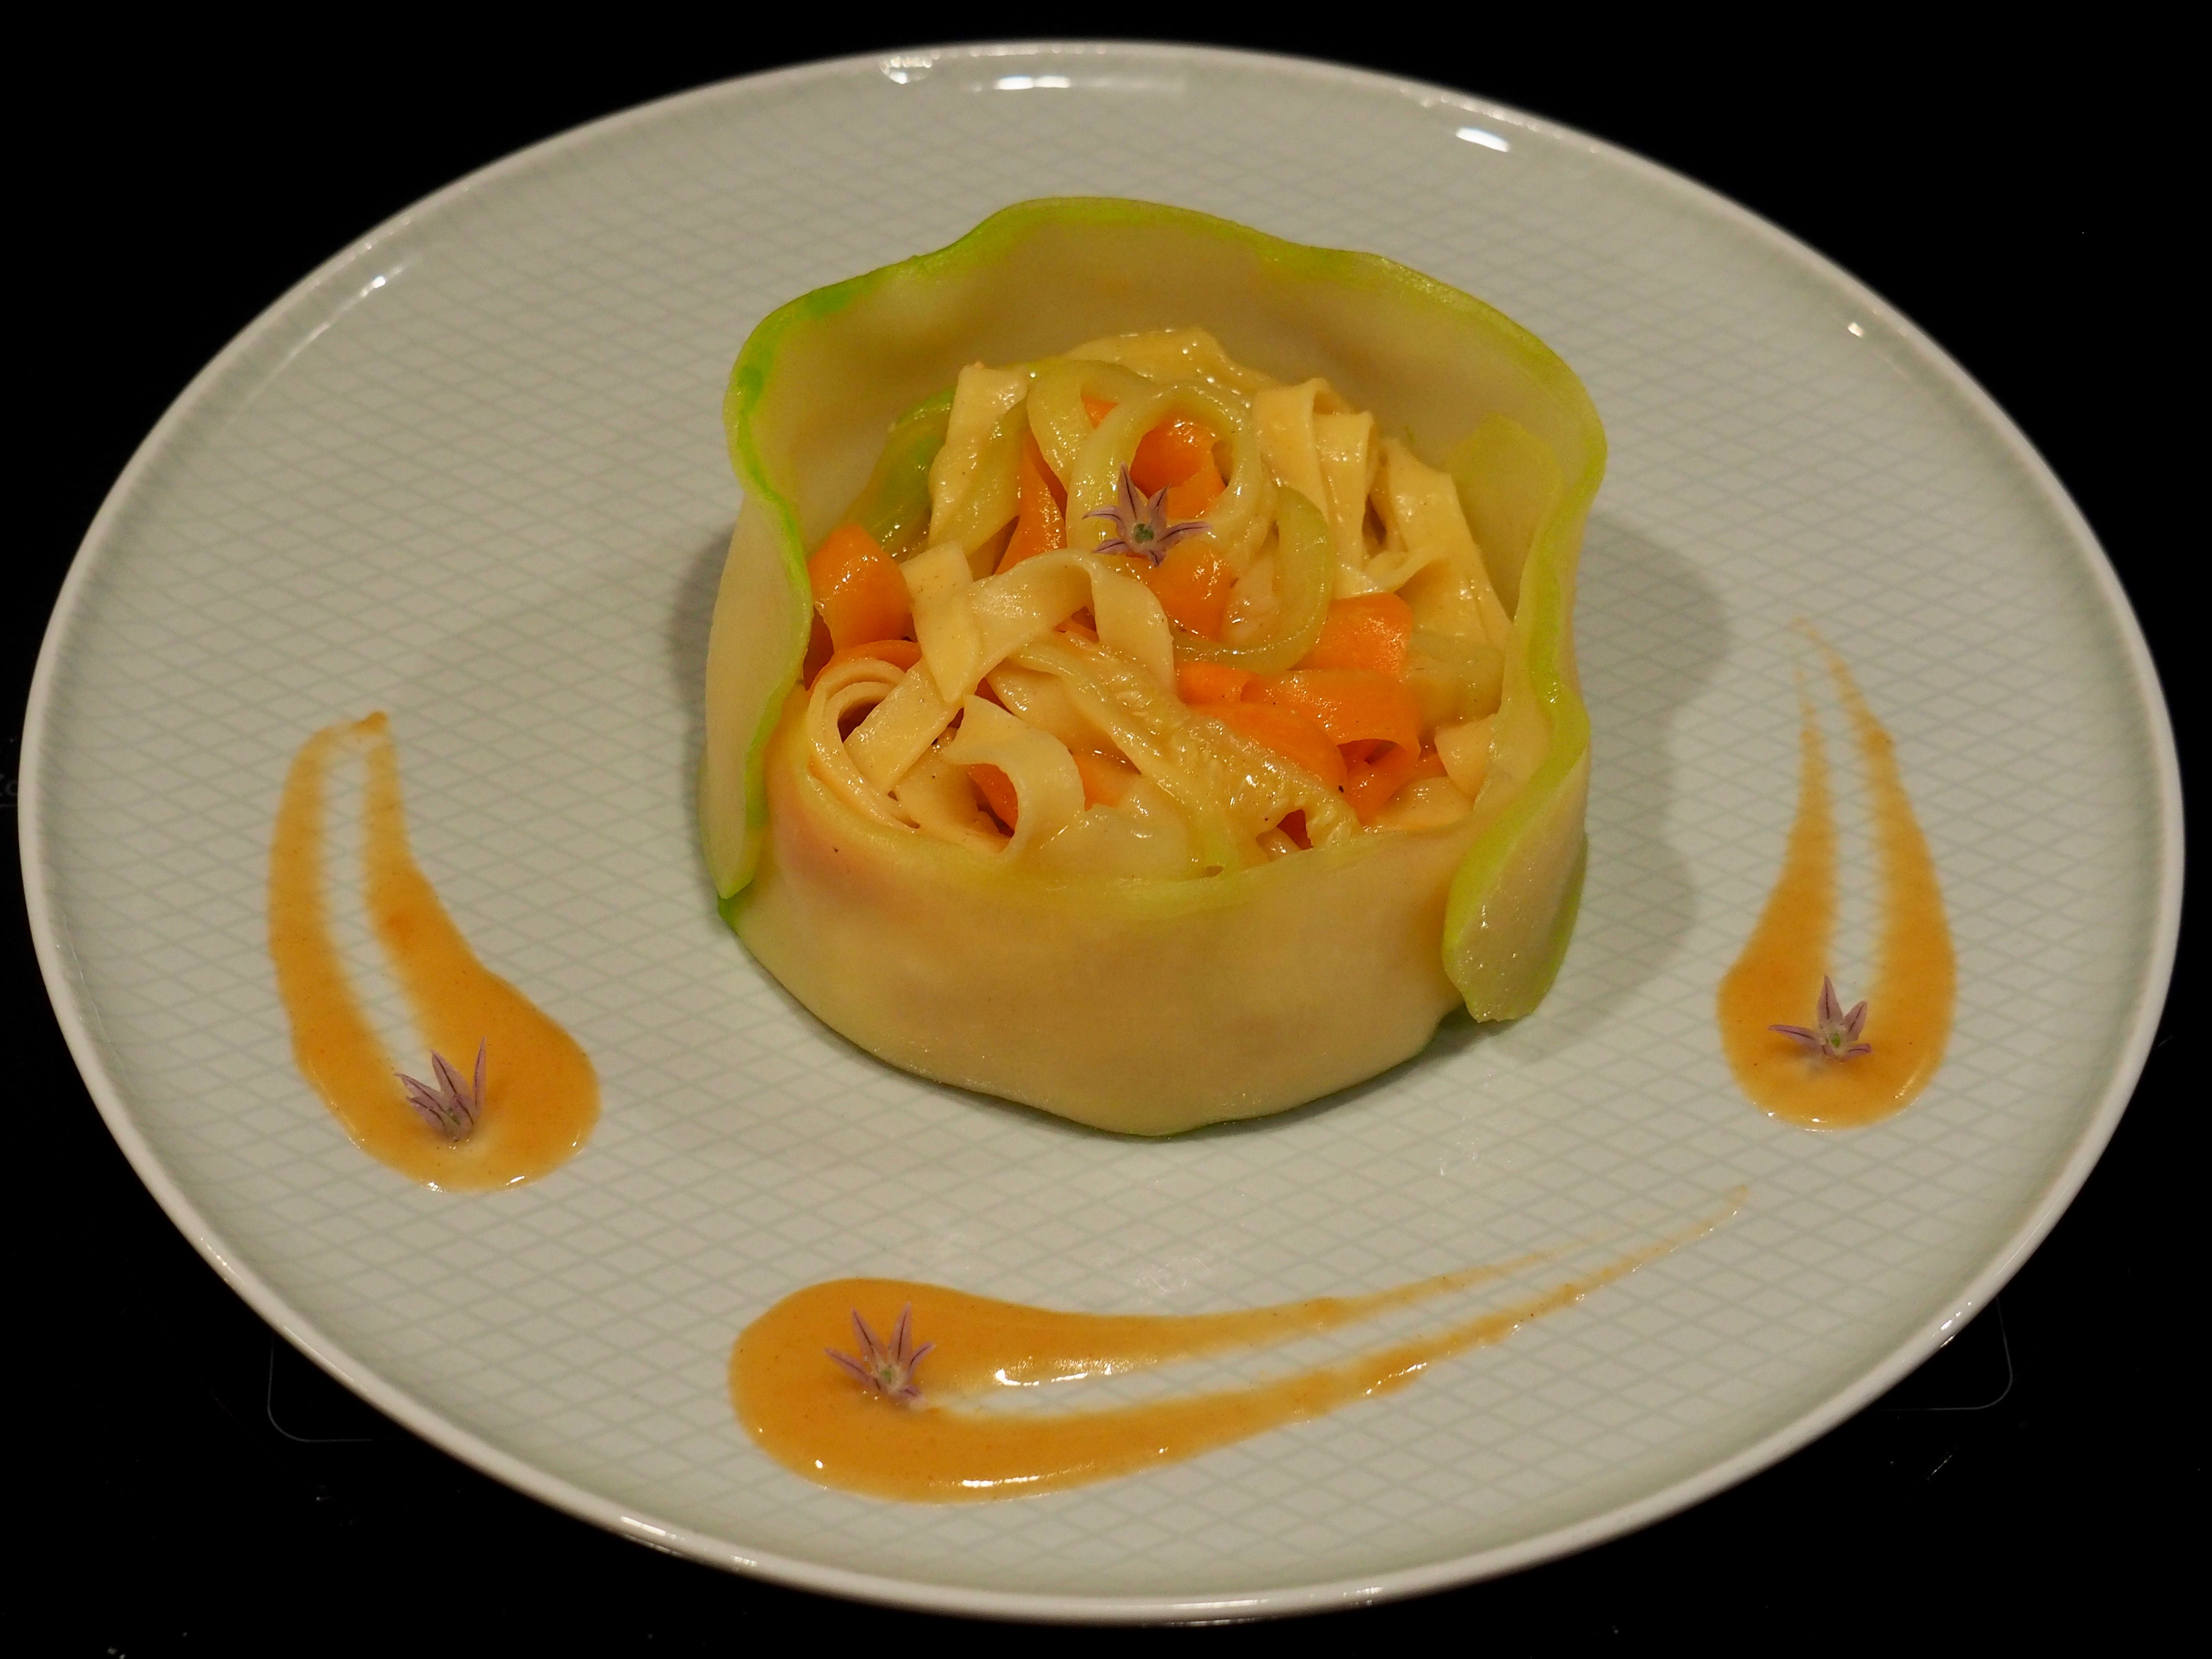
\includegraphics[width=0.9\linewidth]{photos/tagliatelles_crevettes} \end{center}

\hypertarget{gnudi-cresson-et-ricotta}{%
\subsection*{\texorpdfstring{{\emph{Gnudi} cresson et ricotta}}{Gnudi cresson et ricotta}}\label{gnudi-cresson-et-ricotta}}
\addcontentsline{toc}{subsection}{{\emph{Gnudi} cresson et ricotta}}

\begin{salebox}
\textbf{2 personnes \textbar{} Temps préparation : 15 min \textbar{}
Temps cuisson : 15 min \textbar{} Temps repos : 30 min}

Vous connaissiez les \emph{gnocchi}, vous aimerez les \emph{gnudi} !
\end{salebox}

\textbf{Ingrédients}

\begin{itemize}
\tightlist
\item
  1 botte de cresson
\item
  250g de ricotta
\item
  1 oeuf
\item
  2 cs de panure
\item
  2 cs de farine
\item
  Le zeste d'un demi citron
\item
  1 gousse d'ail
\item
  25g de beurre
\item
  Un peu de fromage à râper: parmesan idéalement, vieille mimolette\ldots{}
\end{itemize}

\textbf{Consignes}

\begin{itemize}
\tightlist
\item
  Laver et trier le cresson, en enlevant le plus gros de tiges
\item
  Faire tomber les feuilles de cresson en les faisant chauffer dans une casserole
\item
  Les laisser s'égoutter puis les hacher finement
\item
  Le mélanger avec la ricotta puis rajouter l'œuf, la panure et enfin la farine
\item
  Bien mélanger, assaisonner et laisser reposer 30 min au réfrigérateur
\item
  Dans une assiette, verser un peu de farine puis former des petites sphères avec la pâte (de la forme de gnocchi) et les passer dans la farine pour les enrober (si la préparation est trop collante rajouter un peu de farine dans la préparation mais elle doit quand même rester un peu collante)
\item
  Faire chauffer une grande quantité d'eau et une fois à ébullition, plonger les gnudi délicatement dedans. Lorsqu'il remonte à la surface c'est qu'ils sont cuits.
\item
  Pendant la cuisson, faire chauffer dans une sauteuse le beurre et y faire revenir l'ail et le zeste de citron
\item
  Lorsque les gnudi sont cuits, les sortir de l'eau à l'aide d'une écumoire et les mettre directement dans le beurre
\item
  Les faire revenir quelques minutes dans le beurre puis servir
\item
  Agrémenter de parmesan/mimolette vieillie
\end{itemize}

\begin{center}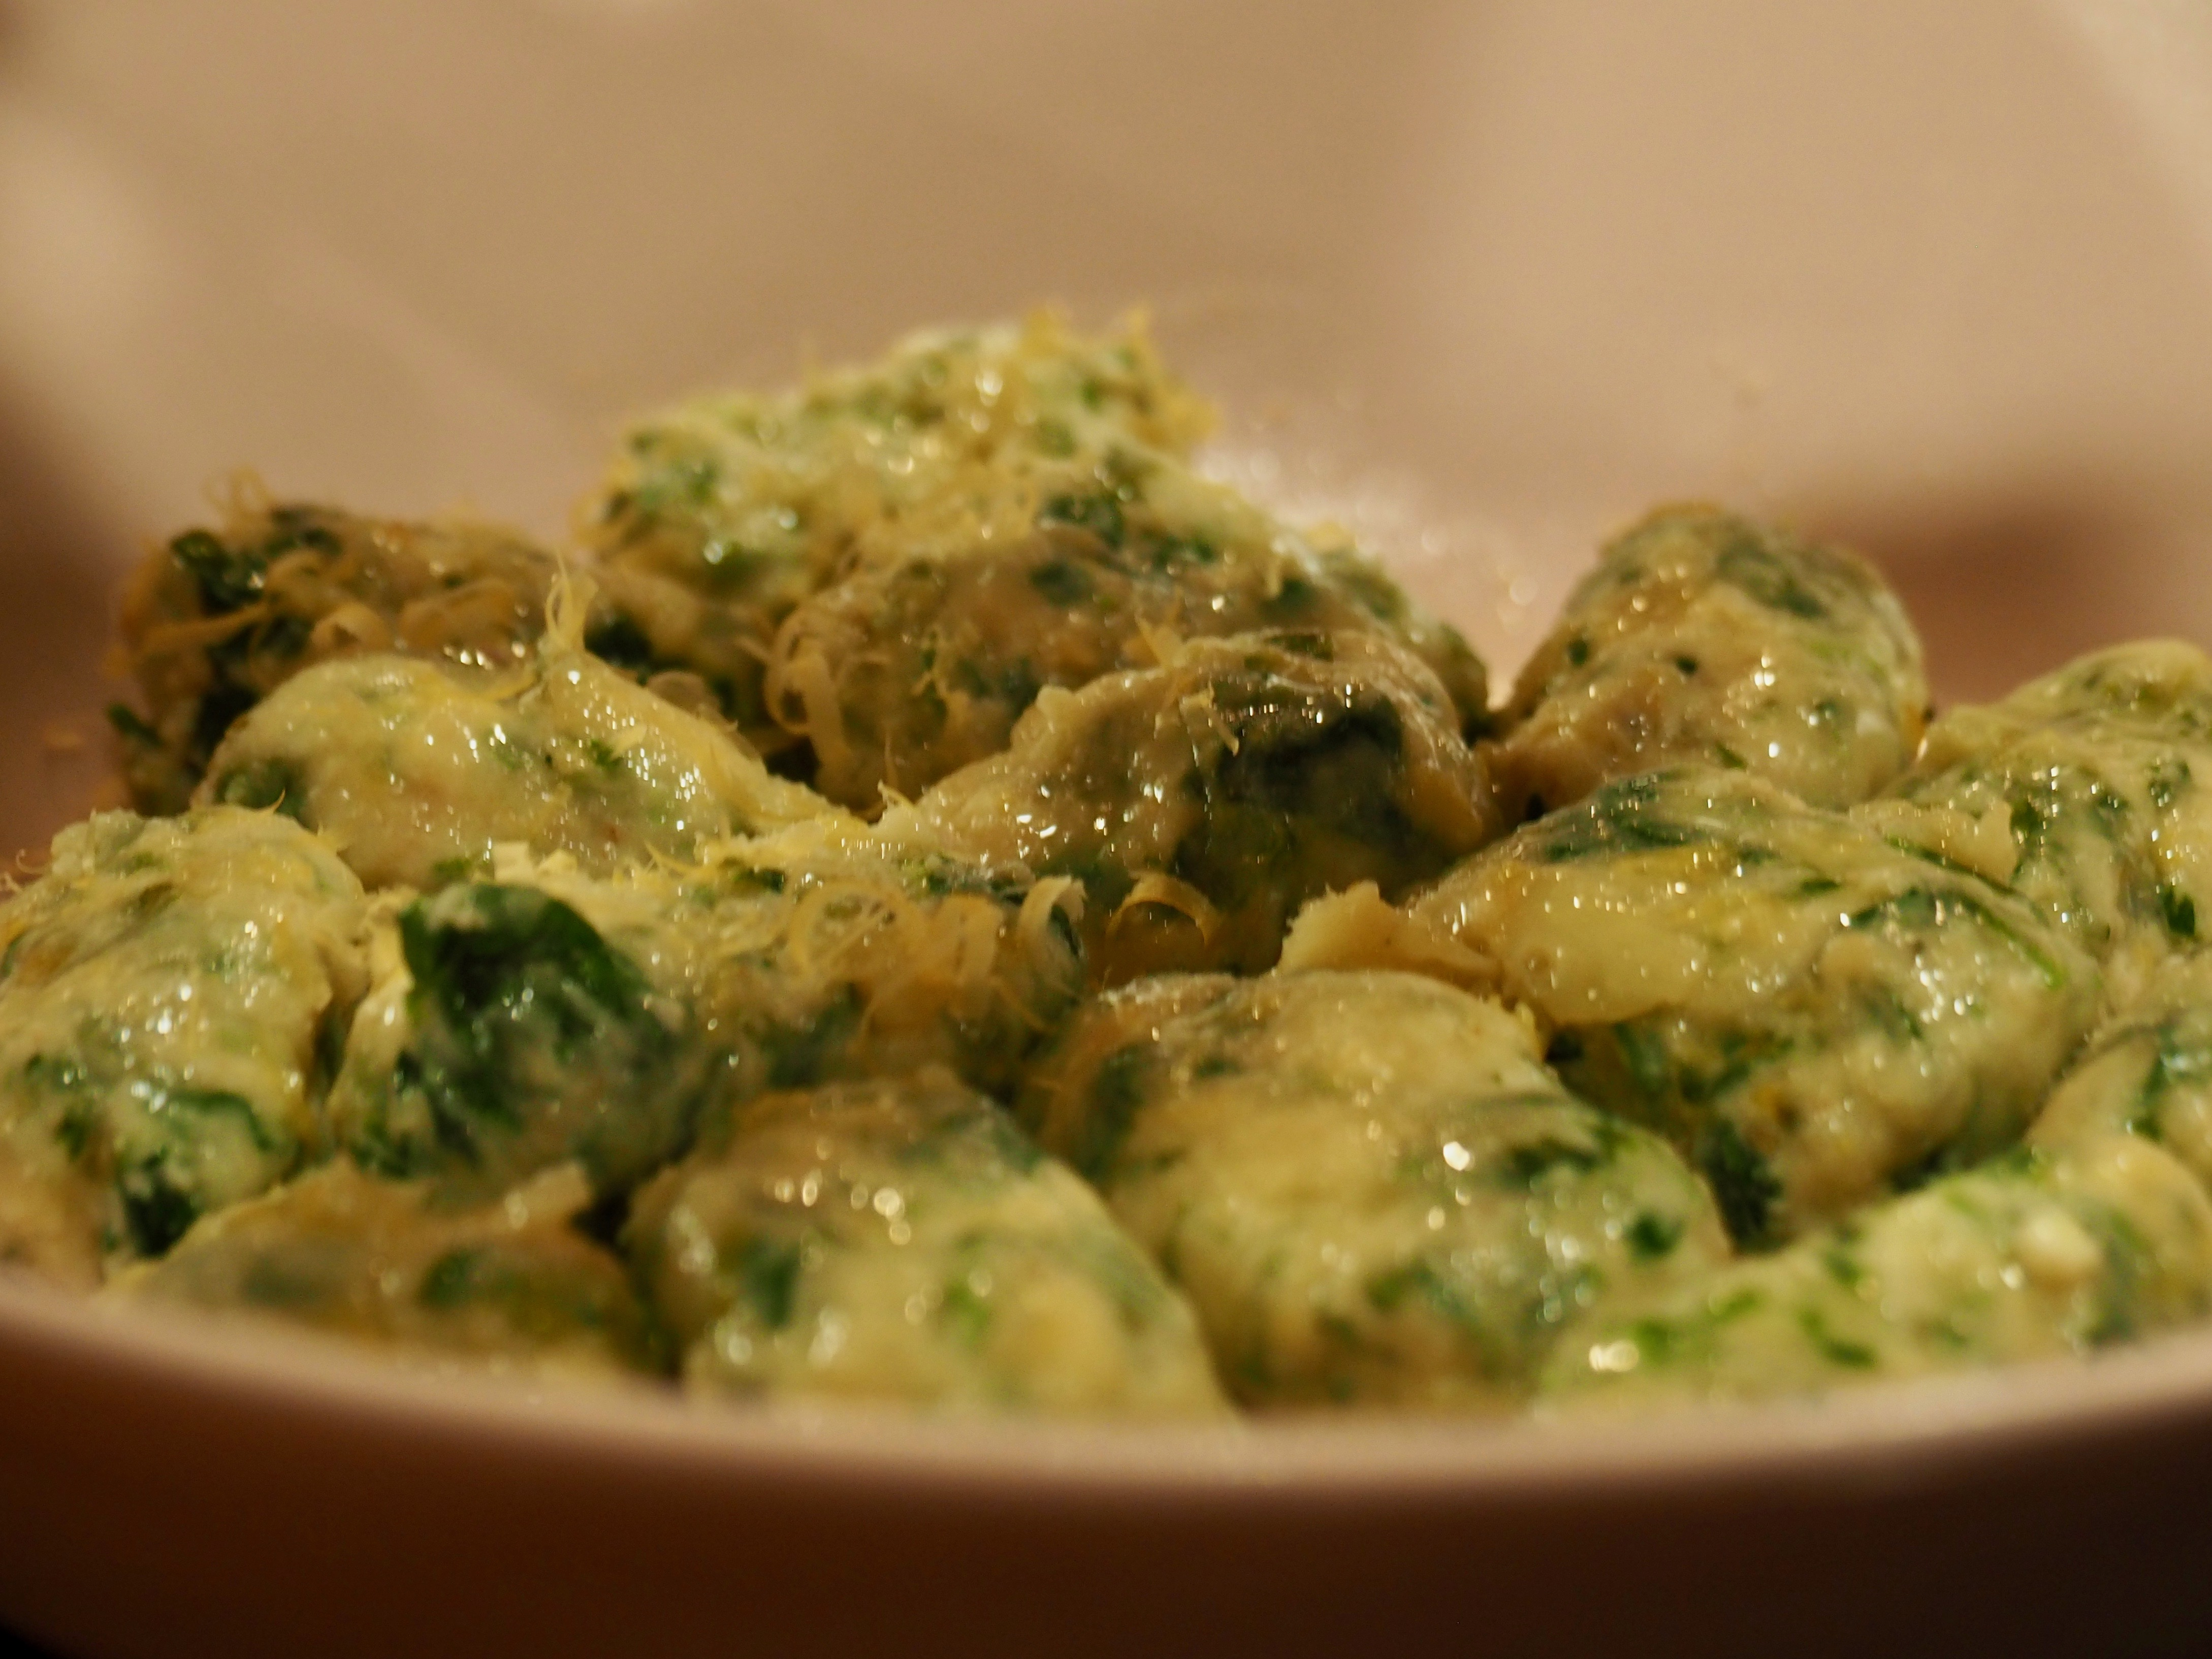
\includegraphics[width=0.9\linewidth]{photos/gnudi} \end{center}

\begin{center}\rule{0.5\linewidth}{0.5pt}\end{center}

\begin{center}\rule{0.5\linewidth}{0.5pt}\end{center}

\hypertarget{sucruxe9-1}{%
\section*{Sucré}\label{sucruxe9-1}}
\addcontentsline{toc}{section}{Sucré}

\hypertarget{tartelettes-citron-menthe-sans-cuisson}{%
\subsection*{\texorpdfstring{{Tartelettes citron-menthe sans cuisson}}{Tartelettes citron-menthe sans cuisson}}\label{tartelettes-citron-menthe-sans-cuisson}}
\addcontentsline{toc}{subsection}{{Tartelettes citron-menthe sans cuisson}}

\begin{sucrebox}
\textbf{4 tartelettes (10 cm) \textbar{} Temps préparation : 40 min
\textbar{} Temps cuisson : 0 min \textbar{} Temps repos :
\textasciitilde{} 2h}

Recette intégralement sans cuisson
\end{sucrebox}

\textbf{Ingrédients}

\begin{itemize}
\tightlist
\item
  85 g de flocons d'avoine
\item
  45 g de noisettes (ou d'amandes)
\item
  65 g d'huile de coco
\item
  85 g de dattes ou de pruneaux
\item
  3 citrons
\item
  3 oeufs
\item
  2 gouttes d'huile essentielle de menthe poivrée
\item
  Quulques feuilles de menthe
\item
  4 cuillères à soupe de sucre (suivant goûts)
\item
  1 g de gélatine
\item
  20 g de beurre
\end{itemize}

\textbf{Consignes}

\begin{itemize}
\tightlist
\item
  Mixer les flocons d'avoine et les noisettes jusqu'à obtenir une poudre
\item
  Rajouter les dattes et l'huile de coco (amollie ou fondue) puis mixer à nouveau jusq'à obtenir une consistance pateuse
\item
  Foncer la pâte dans des cerles à tartelettes préalablement chemisés de filme alimentaire. Bien marquer les pourtours. Laisser prendre au frais au moins une heure
\item
  Faire chauffer le jus et le zeste des citrons avec le sucre, les oeufs battus et les deux gouttes d'huile essentielle. Bien remuer jusq'à épaisissement
\item
  Sortir du feu et ajouter le beurre et la gélatine (réhydratée) avant d'homogénéiser
\item
  Couler l'appareil dans les fonds de tartes et remettre à prendre au frais
\item
  Décorer de quelques feuilles de menthe
\end{itemize}

\begin{center}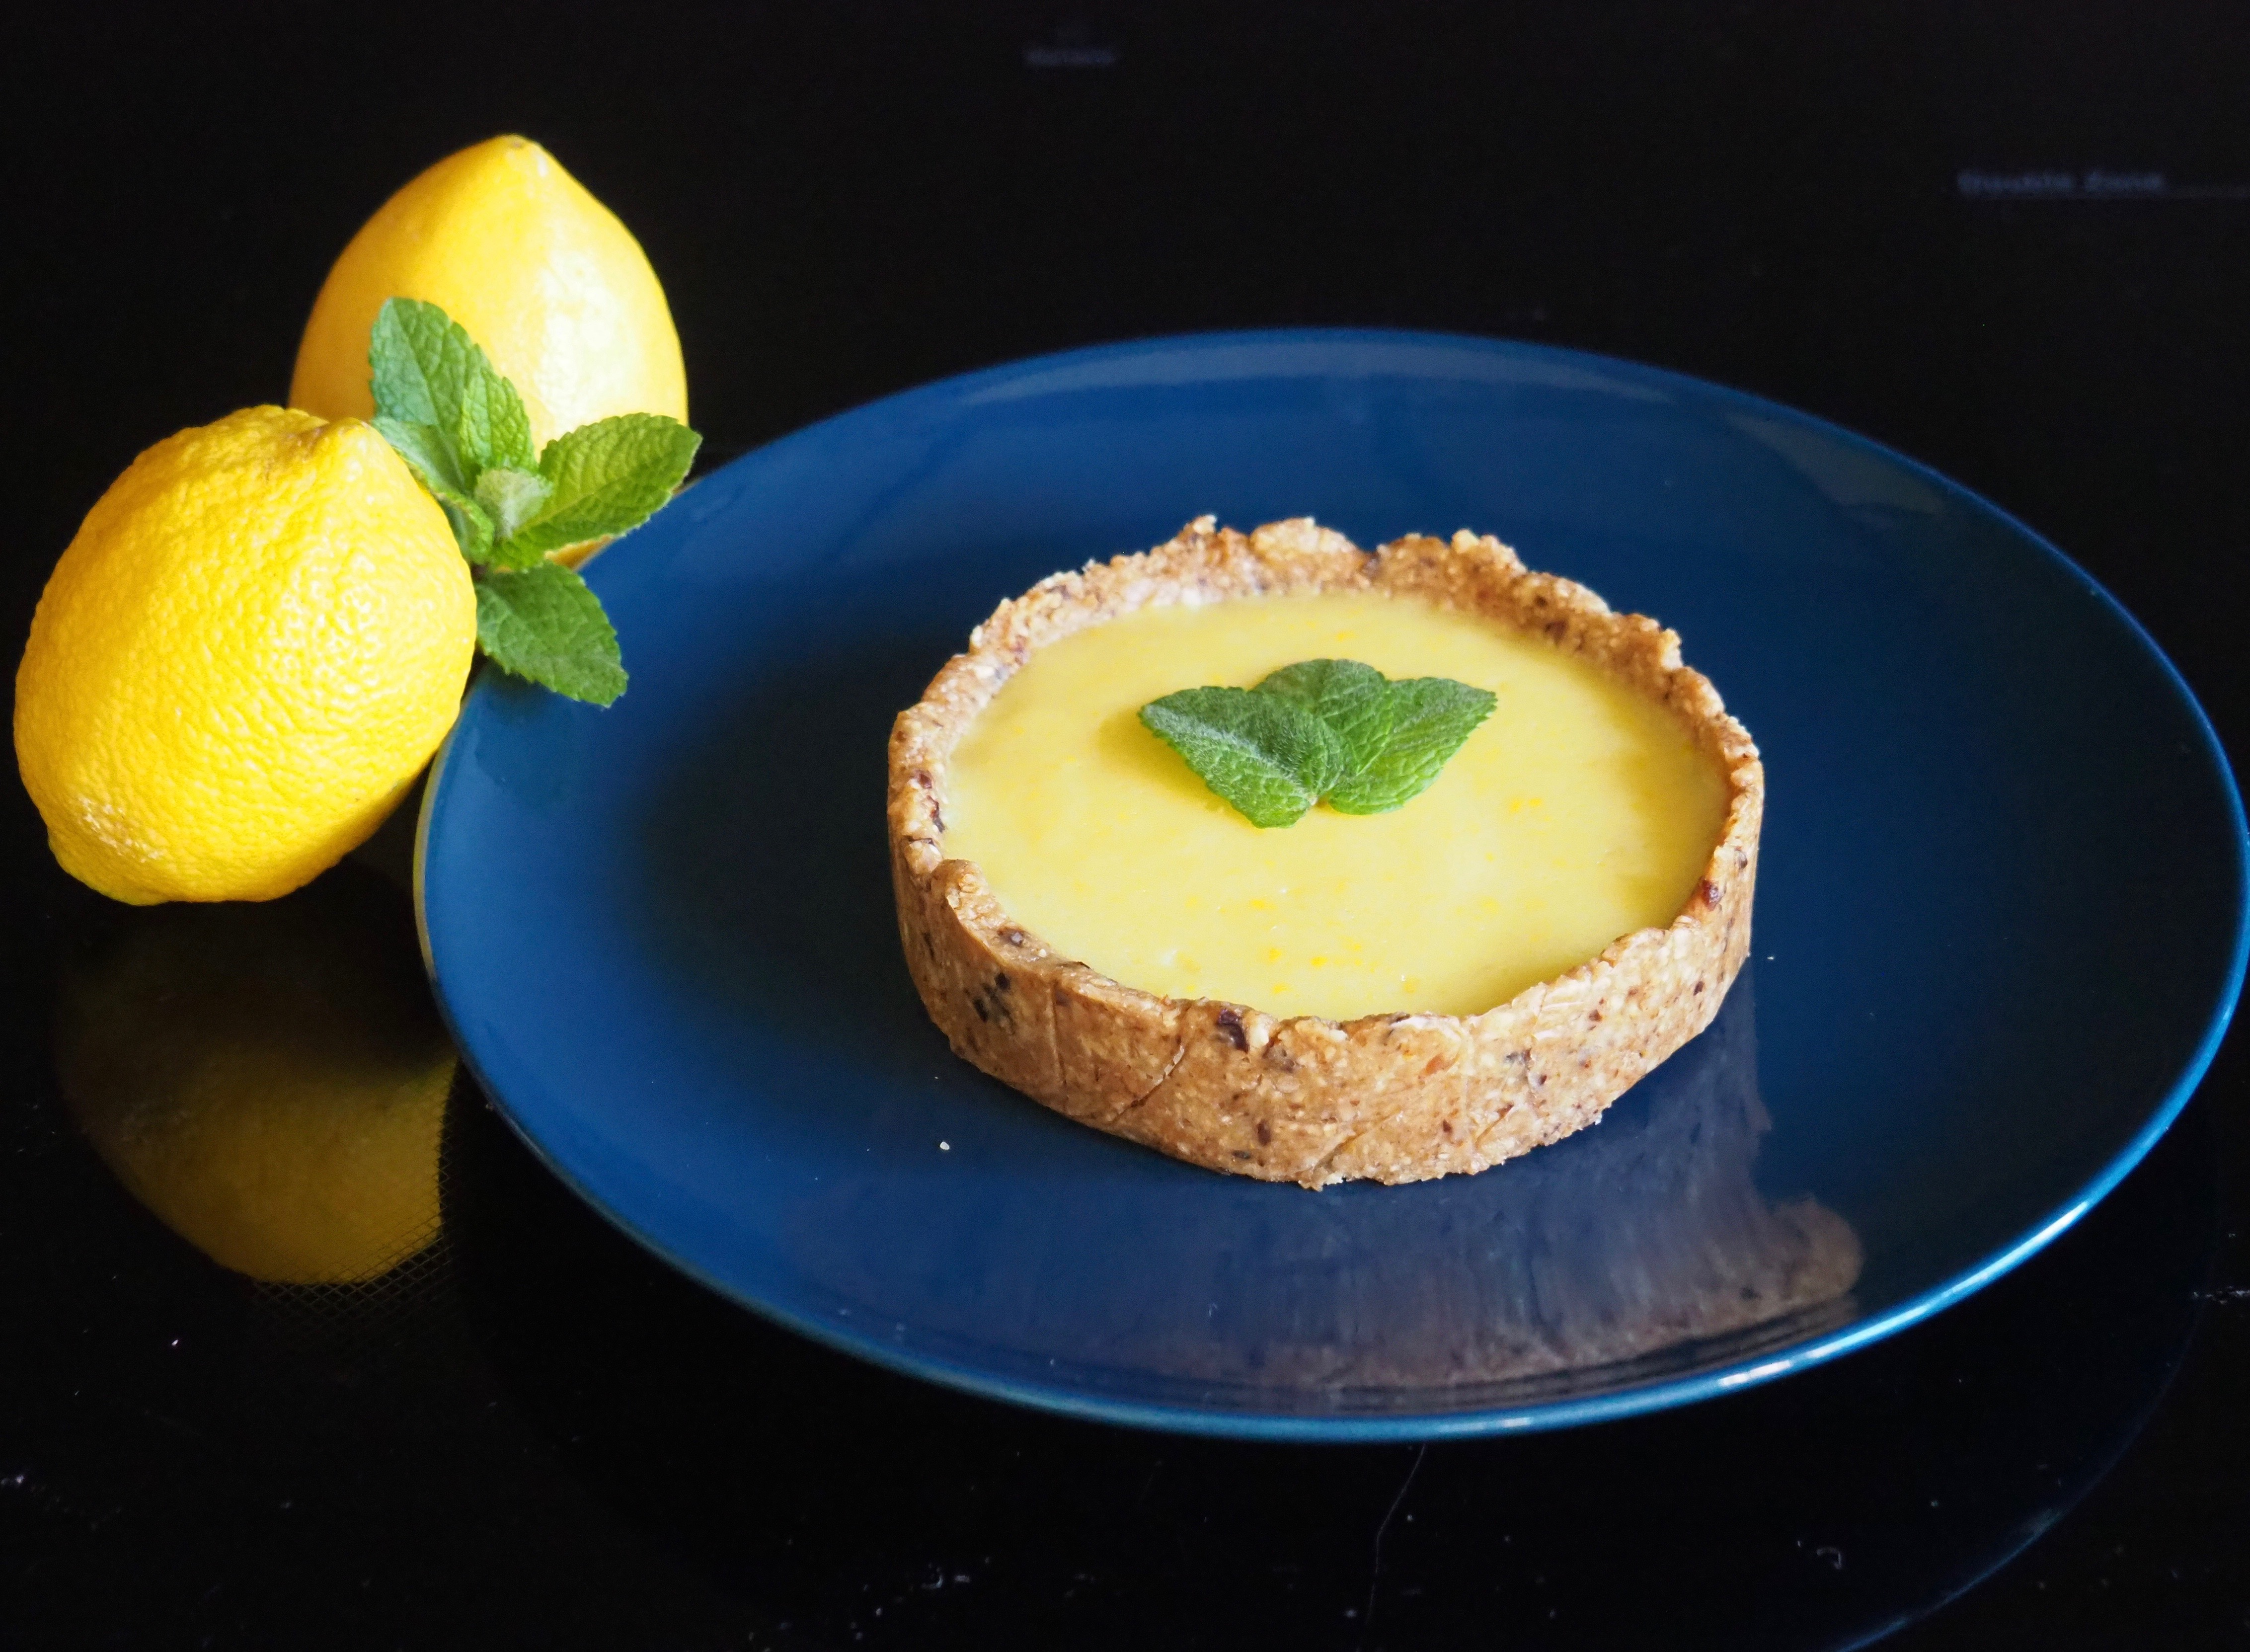
\includegraphics[width=0.9\linewidth]{photos/citron_menthe} \end{center}

\begin{center}\rule{0.5\linewidth}{0.5pt}\end{center}

\end{document}
